%!TEX root = ../dokumentation.tex

\chapter{Result}

\section{Outsourcing of Apache Kafka Client}

The first task for the movement of the car sharing app to a cluster instead of a local setup was to oursource the kafka client to the IBM Cloud Message Hub. Basically this needed a few configurations of the kafka client inside the car sharing app as decsribed in chapter 3.x. Because yet there is no app with which the functionality could have been tested it was necessary to create a test application, with which the producing as well as the consuming of messages can be tested.

This app has three different text fields in total - One for specifying the topic of the message to produce. Another one for the key of the message and a third one for the value. With the submit button this message will be produced to the defined topic.

Additionally there are two predefined topics - confirm and booking . and for each of them a consumers is running in another thread. The consumers are continiously listening for newly produced messages for those topics. If one of them consumes a new message while it is running this message is shown below the matching header.

How the app looks like can be seen in the figure below.

\begin{figure}[h]
\centering
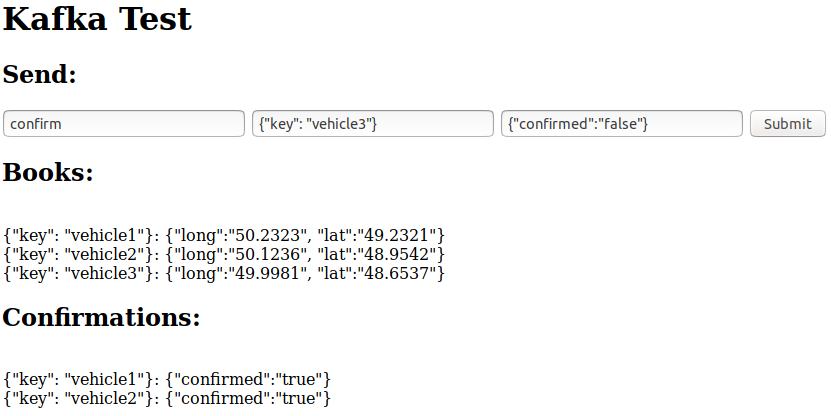
\includegraphics[width=\textwidth/5*4]{images/kafka_test_ui.png}

\textsuperscript{Figure 4.1.1 Kafka client test Web App}\\
\end{figure}

With this testing app also the DummyScheduler can be tested. When producing a message for the booking topic in a JSON format the DummyScheduler mirrors this message to the confirm topic. This means it produces an equal message for the confirm topic. Because the test app also includes a consumer for this topic and prints the consumed messages on the web app the mirrored message can be seen there, if the DummyScheduler is working. If there is no new message for confirm topic a few seconds after the book message got produced, the DummyScheduler is not working correctly.

All in all this way the app enables testing both - the outsourcing of the Kafka client itself and the correct functionality of the DummyScheduler.

\section{Communication between car sharing app and services}

The movement of the car sharing app from a local setup to a cluster not only changes the location, where the app is running. It also changes the way of communication between the single apps and services. This means this movement did not only needed a setup on a different location, but also some changes of the code for maintaining the communication. 

As described in chapter 4.1 the Kafka client was outsourced to IBM Cloud message hub. The way of communication does not change in general, only some additional configurations like security protocols and access data had to be made and the broker had to be changed from localhost to an online client. Also the topics had to be created in the online client of Kafka as well, so that messages can be consumed as well as produced. After those changes have been made the workflow with Kafka didn't change at all, so that there is no further need of adjustments. The functionality can be tested with the testing web application descibed in chapter 4.1.

The other services - mongo and osrm - weren't necessary for the DummyScheduler, but they were for the real scheduler. Same applies to the cplex engine.

For moving this to the cluster as well, first it was necessary to isolate the needed part of the cplex engine - the python library installer - and copy it inside the docker container to be created. Inside of this docker container this cplex python library is automatically installed, which enables all needed functionalities directly inside the created docker container.

The mongo and osrm services had already basic images available, on which could be built up. They got extended by the necessary data and also by preprocessing those data for restoring the database in case of mongo or preparing the map in case of osrm. Those extended docker containers were also deployed on the cluster.

The communication inside a cluster is working differently from a communication on a local device. Even if the deployments are running inside the same network, as described in chapter 2.2, it is necessary to create services for allowing the deployments to talk to each other. Then the host has to be changed from local host to the name of the service, to which it has to be talking to.

%check described in 2.2s

The DummyScheduler, the simulation client and the simulation server are running on different containers on the cluster. In two other additional containers the mongo and the osrm containers are running. The DummyScheduler only needs the KafkaClient for its calculations. That's why it only accesses the Kafka client on IBM Cloud Message Hub, which is not deployed on the cluster but on IBM Cloud.

The simulation client doesn't get real requests via the Kafka client, but predefined ones of a JSON file located in the project itself. That's why it needs no connection to the Kafka client. Instead it accesses the OSRM service for calculating the route for the vehicles to the customers. For optimizing the scheduling it also uses the cplex engine installed inside the docker container. The results are then written to the MongoDB, which is the reason why it has to access the mongo container too. 

The simulation server only reads from the Mongo database for returning the current state of the simulation. The service of the simulation server is exposed with an ingress as described in chapter 3.x. That's how an external client can access the simulation server, for example a demo UI. This demo UI can then visualize the state of the simulation as can be seen in the picture below.

\begin{figure}[h]
\centering
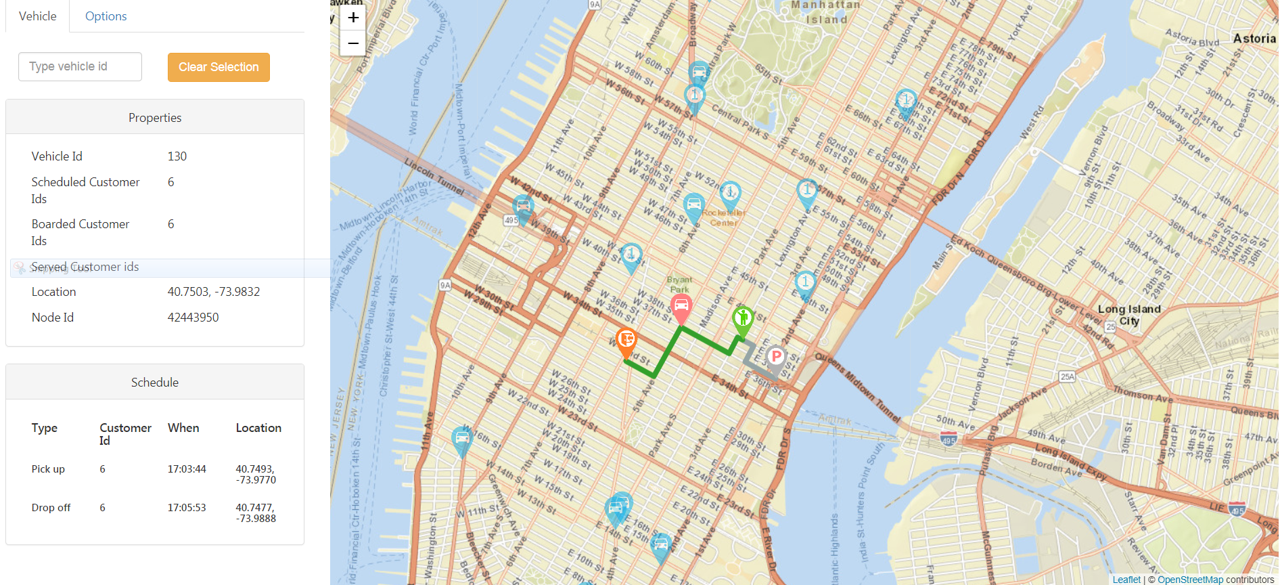
\includegraphics[width=\textwidth/5*4]{images/simulation_ui.png}

\textsuperscript{Figure 4.2.2 Simulation User Interface}\\
\end{figure}

Those results will be compared to the formulated criteria in chapter 3.1 in the next chapter 5.